\documentclass[11pt]{article}
\usepackage{graphicx}
\usepackage{hyperref}
\usepackage{appendix}
\usepackage{amsmath}
\usepackage{amsthm}
\usepackage{amssymb}
\usepackage[moderate]{savetrees}
\usepackage{float}
\usepackage{multirow}
\usepackage{commath}
\usepackage{wrapfig}
\usepackage{booktabs}
\usepackage{subcaption}
\renewcommand{\arraystretch}{1.2}
\usepackage{siunitx}
\sisetup{detect-all}
\usepackage{listings}
\usepackage{color} %red, green, blue, yellow, cyan, magenta, black, white
\definecolor{mygreen}{RGB}{28,172,0} % color values Red, Green, Blue
\definecolor{mylilas}{RGB}{170,55,241}
\usepackage[a4paper,margin=15mm]{geometry}
\numberwithin{equation}{section}
\setlength{\parskip}{\baselineskip}
\setlength{\parindent}{0pt}
\hypersetup{
    colorlinks=true,
    linkcolor=black,
    filecolor=black,      
    urlcolor=black,
    citecolor=black
}
\urlstyle{same}
\lstset{language=Matlab,%
    %basicstyle=\color{red},
    breaklines=true,%
    morekeywords={matlab2tikz},
    keywordstyle=\color{blue},%
    morekeywords=[2]{1}, keywordstyle=[2]{\color{black}},
    identifierstyle=\color{black},%
    stringstyle=\color{mylilas},
    commentstyle=\color{mygreen},%
    showstringspaces=false,%without this there will be a symbol in the places where there is a space
    numbers=left,%
    numberstyle={\tiny \color{black}},% size of the numbers
    numbersep=9pt, % this defines how far the numbers are from the text
    emph=[1]{for,end,break},emphstyle=[1]\color{red}, %some words to emphasise
    %emph=[2]{word1,word2}, emphstyle=[2]{style},    
}
\begin{document}
\title{\textbf{UCL Mechanical Engineering 2021/2022}\\MECH0024 Coursework}
\author{RFLH9}
\date{\today}
\maketitle
\tableofcontents
\listoffigures
\newpage
\part{SpaceX rocket engine essay}
SpaceX has been developing rocket engines for nearly two decades. The two primary engine families being developed today are the Merlin series and the Raptor series. The Draco and SuperDraco series of engines have also been developed by SpaceX, however their role as Reaction Control System (RCS) thrusters and Launch Abort System engines respectively leave them to be not considered in this essay. SpaceX has developed these rocket engines to power a variety of booster rockets, including the Falcon 9, Falcon Heavy and Starship. The roles of these rockets include delivering crew and cargo to space, as well as interplanetary travel. SpaceX places a strong emphasis on reusability and a reduction of `cost to launch'. Hence, the engines powering these flights must be efficient, powerful and reliable to facilitate multiple missions.

The Merlin series of engines power the Falcon 9 and Falcon Heavy rocket boosters. These are two-stage rockets, primarily designed to place cargo and crew into earth orbit. The first stage is powered by nine Merlin `sea level' engines and the second stage is powered by one Merlin `vacuum' engine. There have been a variety of developments over the past years and the current generation of Merlin engines are the Merlin 1D. The Merlin 1D uses an open-cycle gas-generator cycle with Rocket Propellant 1 (RP-1) and liquid oxygen (LOX) as propellants.

The fuel choice for the Merlin engine is due to a large variety of factors. The Merlin engine uses liquid propellants for combustion. RP-1 is a refined kerosene with low amounts of impurities. This is to prevent stray chemical elements from reacting with engine components and causing a breakdown. RP-1 is a liquid at room temperature, safe to handle, cheap and available in large quantities. This makes it ideal for rockets which need to fly frequently (as the Falcon rockets do). However, RP-1 is not the most efficient fuel as liquid Hydrogen has a far greater specific impulse (\SI{289}{\second} vs \SI{381}{\second}) but RP-1 has greater density (\SI{0.071}{\gram\per\mol} vs \SI{0.82}{\gram\per\mol}) \cite{b1}. A disdvantage of RP-1 is that it is a hydrocarbon, resulting in carbon deposits when burnt at the improper fuel-oxidiser ratio. This can lead to a build up of carbon deposits in the engine, decreasing the lifetime of the engine. Some alternatives to RP-1 include liquid Hydrogen and liquid Methane. These two fuels are sometimes referred to as cryogenic fuels as their boiling points are far below room temperature and require more complex pressurised tanks and plumbing within the engine.

\begin{figure}[H]
    \centering
    \begin{minipage}{.5\textwidth}
        \centering
        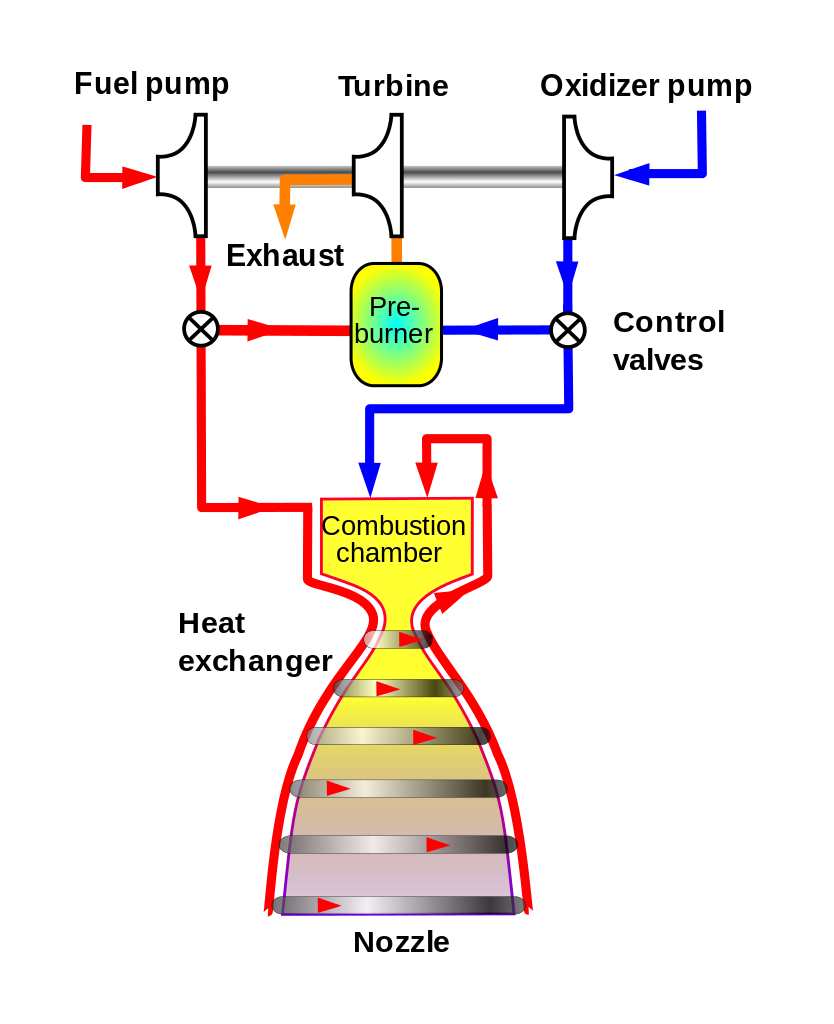
\includegraphics[height = 25ex]{./img/openCycle.png}
        \captionof{figure}{Open-cycle gas-generator cycle \cite{b2}.}
        \label{gasGeneratorCycle}
    \end{minipage}%
    \begin{minipage}{.5\textwidth}
        \centering
        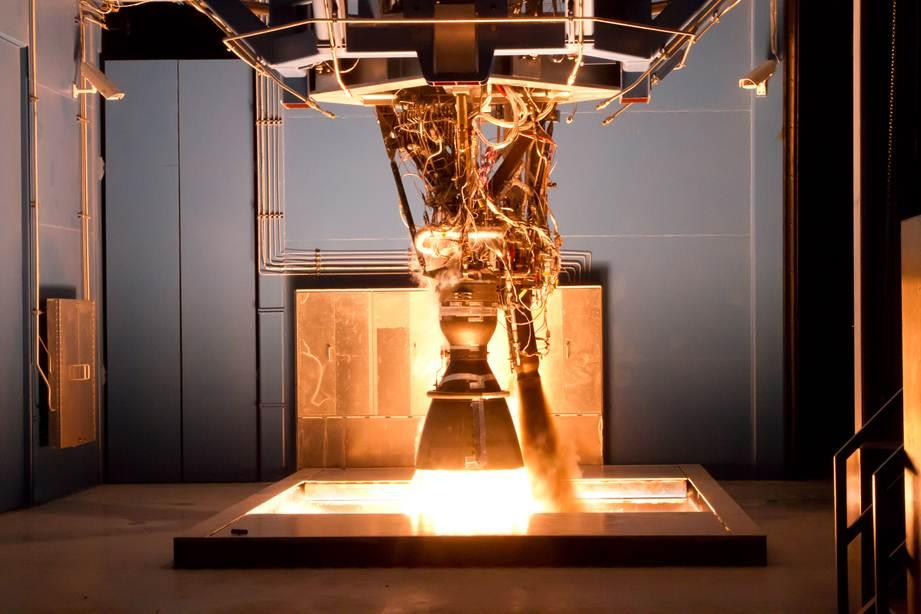
\includegraphics[height = 25ex]{./img/merlinTest.jpg}
        \captionof{figure}{Merlin engine test fire. Note the black exhaust on the right side from the preburner and turbine \cite{b3}.}
        \label{merlinTest}
    \end{minipage}
\end{figure}

To dissect the combustion cycle of the Merlin engine, let us take a look at how the engine is designed. In Figure \ref{gasGeneratorCycle}, we see that RP-1 and LOX is fed through turbopumps powered by an impeller on a single shaft. This shaft is powered by a turbine. This is driven by gases from a `preburner', where some of the propellants are combusted and the hot gas is used to turn the shaft, powering the fuel and oxidiser pumps. The products of the preburner combustion are not used in the main combustion chamber and hence these products are lost. This is referred to as an open-cycle. The Merlin engine runs its preburner fuel rich and we see evidence of this in Figure \ref{merlinTest} as the exhaust is black with soot.

To improve the efficiency of this cycle, we can feed the exhaust from the preburner into our main combustion chamber `closing our cycle'. This presents an engineering problem in the form of higher back-pressures within the whole system. When the main combustion chamber exerts pressure through to the turbine and pre-burner, this can damage components. To solve this, the preburner needs to generate more energy and higher pressures. The turbine will need to withstand higher temperatures and larger stresses. As seen with the Merlin engine, running the preburner fuel rich reduces the combustion temperature, reducing the stress on the turbine. Depending on the fuel, running fuel rich may result in the formation of carbon deposits within the engine but running oxidiser rich presents an exhaust which is chemically corrosive, due to the presence of high temperature oxygen. However, closing the cycle and its complexity adds weight and points of failure, hence a balance must be struck to ensure that the cycle is more effective.

\begin{figure}[H]
    \centering
    \begin{minipage}{.5\textwidth}
        \centering
        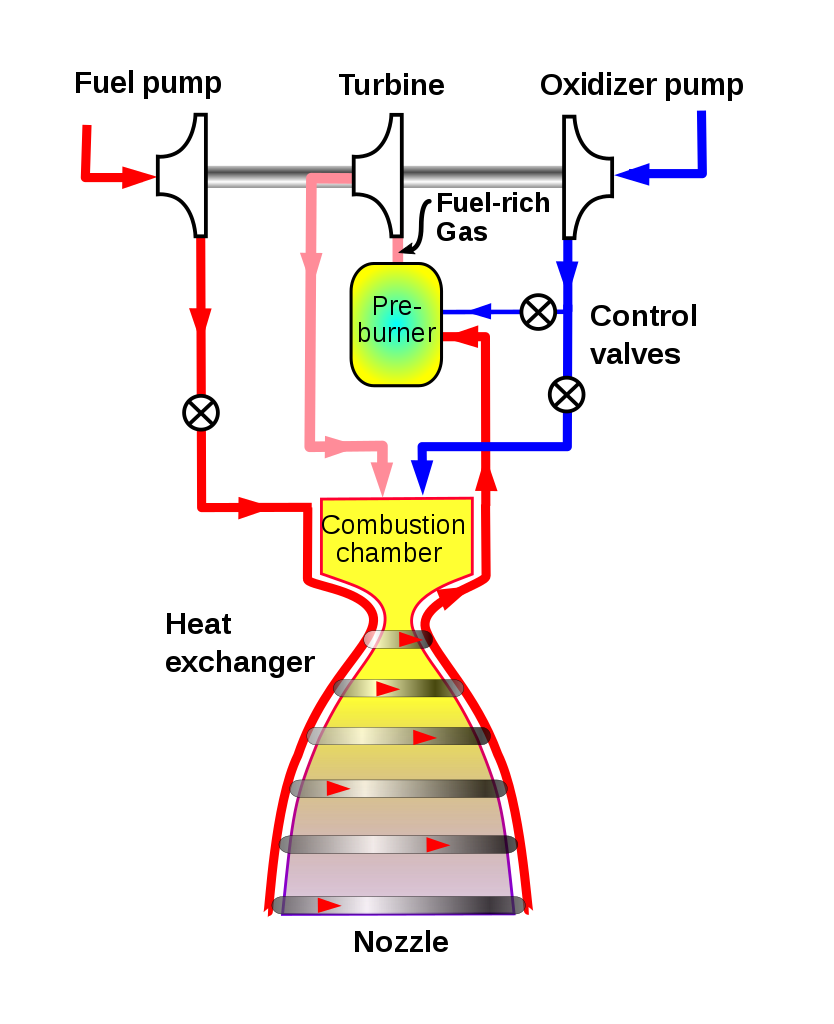
\includegraphics[height = 25ex]{./img/closedCycle.png}
        \captionof{figure}{Closed-cycle staged combustion cycle \cite{b4}.}
        \label{closedCycle}
    \end{minipage}%
    \begin{minipage}{.5\textwidth}
        \centering
        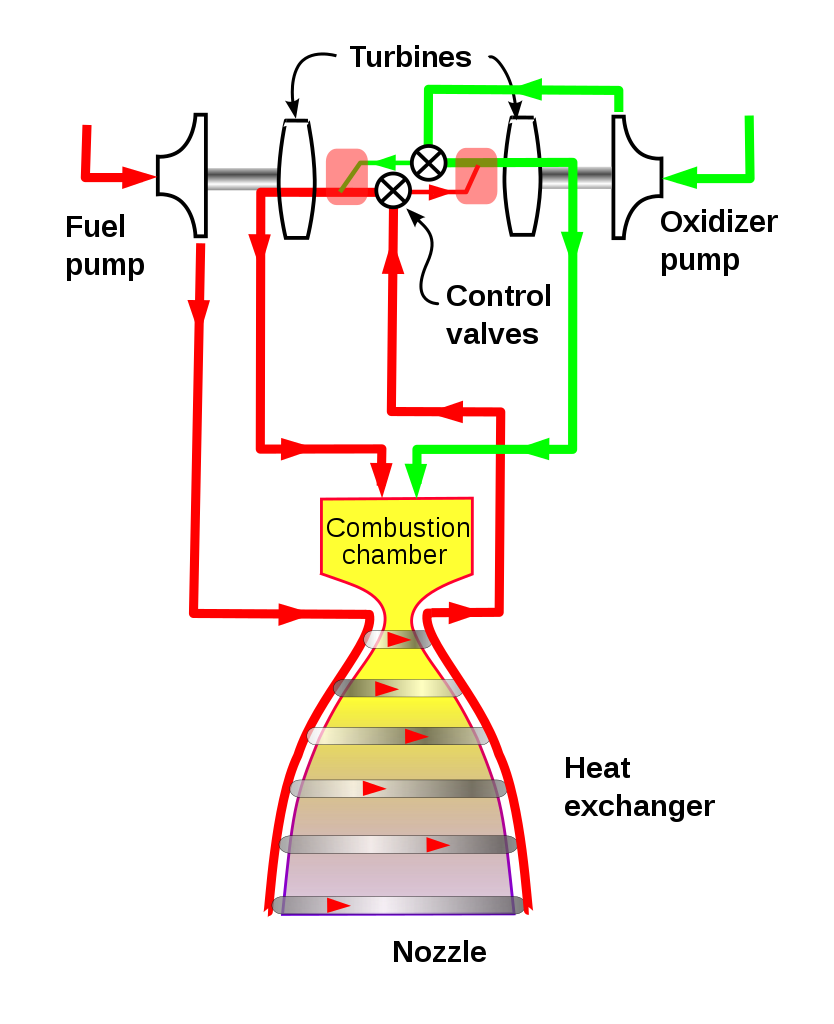
\includegraphics[height = 25ex]{./img/fullFlowCycle.png}
        \captionof{figure}{Full-flow staged combustion cycle \cite{b5}.}
        \label{fullFlow}
    \end{minipage}
\end{figure}

\part{Sea Level and Vacuum Merlin 1D rocket engines analysis}
\section{}
\subsection{Estimation of ideal OF ratio \& comparison with typical value}
test
\subsection{Estimation of isentropic index $\gamma$}
test
\subsection{Estimation of molecular weight of combustion products $M_g$}
test
\subsection{Estimation of heat capacity $c_p$}
test
\subsection{Estimation of the adiabatic flame temperature of the combustion product in the combustion chamber}
test
\section{Determination of mass flux through both rocket engines}
test
\section{Estimation of exit velocity of jet exhaust in both cases}
test
\section{Estimation of exit pressure of the exhaust in both cases}
test
\section{}
\subsection{Estimation of  rocket thrust for the Sea Level Merlin 1D during the initial take-off and the Vacuum Merlin 1D operating in space}
test
\subsection{Estimation of the specific impulse in both cases}
test
\subsection{Discussion of differences between estimations and reported values}
test
\section{Sketch of exit flow/shock expansion fan characteristics}
\subsection{At sea level}
test
\subsection{At an altitude of \SI{5.5}{\kilo\meter}}
test
\section{Description of other technologies (and their working principles), which accommodate the change in back-pressure on thrust performance}
test
\begin{thebibliography}{00}
    \bibitem{b1} Robert A. Braeunig. (2008) `Rocket Propellants' \url{http://www.braeunig.us/space/propel.htm} Accessed: 14/12/2021
    \bibitem{b2} Duk. (2016) `Gas Generator Rocket Cycle' \url{https://commons.wikimedia.org/wiki/File:Gas_generator_rocket_cycle.svg}; see also \url{https://commons.wikimedia.org/wiki/User:Duk}, CC BY-SA 3.0, Accessed 15/12/2021
    \bibitem{b3} SpaceX. (2012) `Merlin 1D Test Fire' \url{http://www.spacex.com/media-gallery/detail/1661/172}; see also \url{http://www.spacex.com/news/2013/03/26/merlin-engines}, CC0, \url{https://commons.wikimedia.org/w/index.php?curid=46487822} Accessed: 15/12/2021
    \bibitem{b4} Duk. (2017) `Staged Combustion Cycle' \url{https://commons.wikimedia.org/wiki/File:Staged_combustion_rocket_cycle.svg#filelinks}; see also \url{https://commons.wikimedia.org/wiki/User:Duk}, CC BY-SA 3.0, Accessed 15/12/2021
    \bibitem{b5} Duk. (2021) `Staged Combustion Cycle' \url{https://commons.wikimedia.org/wiki/File:Full_flow_staged_rocket_cycle.svg}; see also \url{https://commons.wikimedia.org/wiki/User:Duk}, CC BY-SA 3.0, Accessed 15/12/2021
\end{thebibliography}
\end{document}